\thispagestyle{empty}
\null
\vfill
\begin{center}
  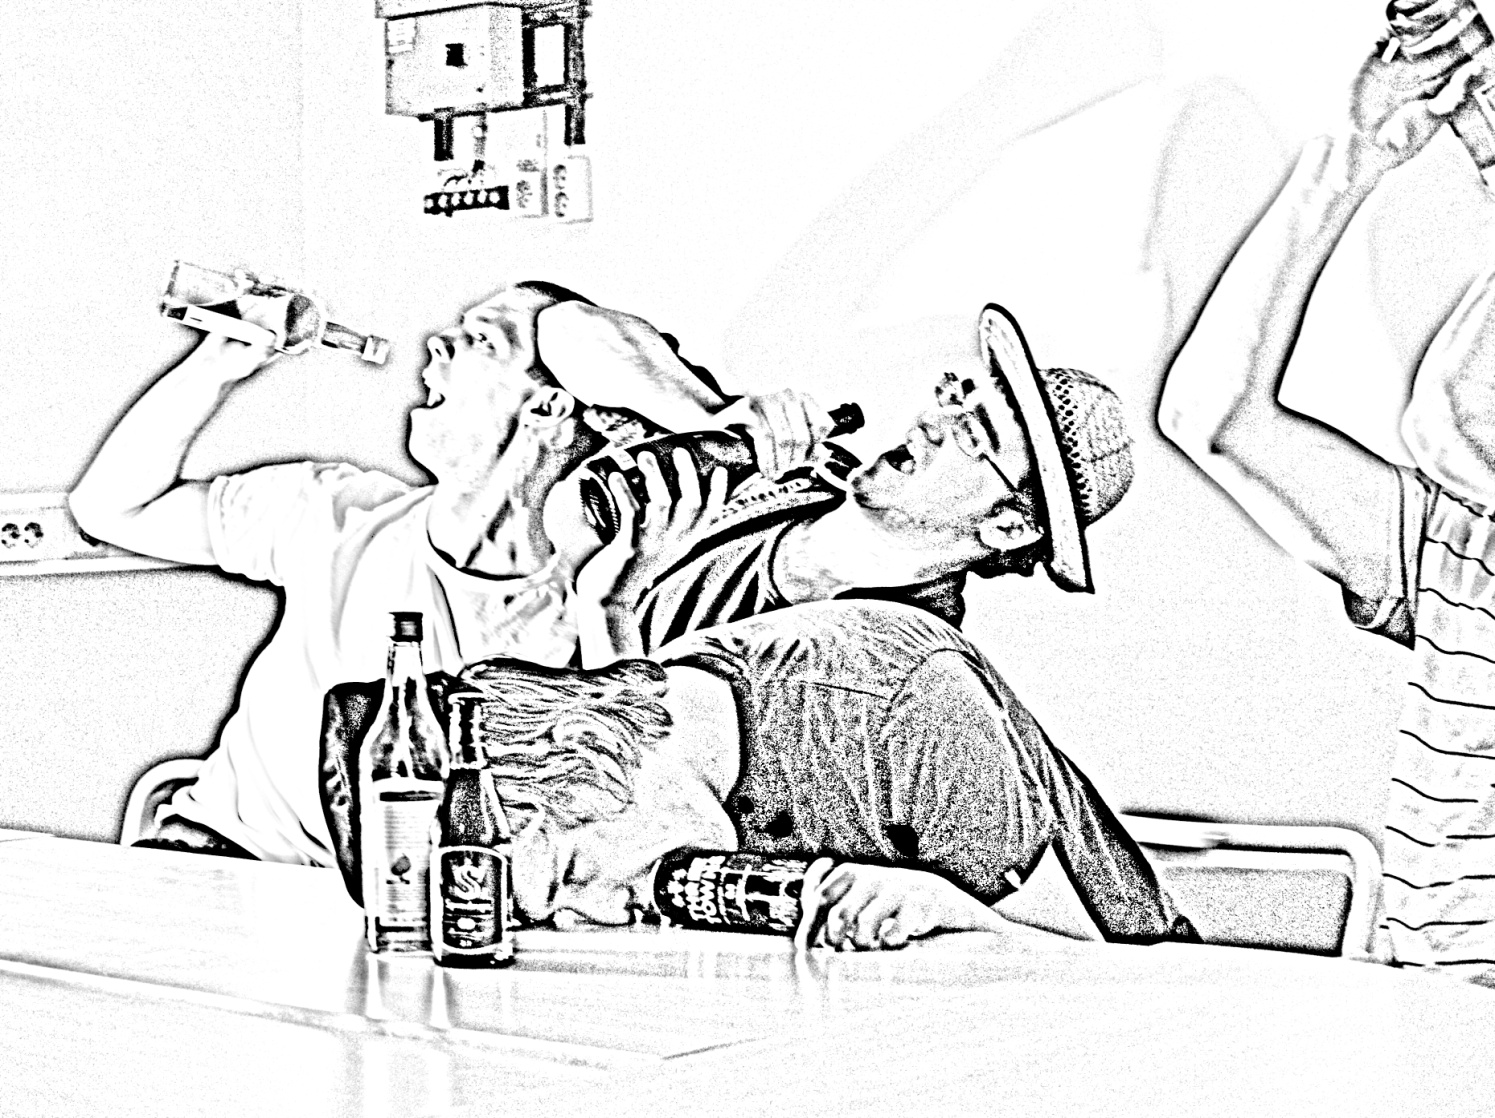
\includegraphics[width=1.0\textwidth]{res/bordsvisor.png}
  \section{Bordsvisor}
\end{center}
\vfill
\newpage


\subsection{Måltidssång (Fredmans epistel nr 21)}
\index[alfa]{Måltidssången (Fredmans epistel nr 21)}
\index[anfa]{Så lunka vi så småningom...}
\textit{Mel: Måltidssång\\skriven av Carl Michael Bellman}\\
\begin{parse lines}[\noindent]{#1\\}

Så lunka vi så småningom
från Bachi buller och tumult.
När döden ropar: Granne, kom,
ditt timglas är nu fullt!
Du gubbe fäll din krycka ner
och du, du yngling lyd min lag:
Den skönsta nymf som åt dig ler
inunder armen tag!

Tycker du att graven är för djup?
Nå, välan, så tag dig då en sup!
Tag dig sen dito en, dito två, dito tre;
så dör du nöjdare.

Säg, är du nöjd, min granne, säg?
Så prisa världen nu till slut!
Om vi har en och samma väg
så följoms åt... Drick ut!
Men först med vinet, rött och vitt,
för vår värdinna bugom oss,
och halkom sen i graven fritt
vid aftonstjärnans bloss!

Tycker du…
\end{parse lines}


\subsection{Fyllevisa}
\textit{Mel: Vi gå över daggstänkta berg}\\
\index[alfa]{Fyllevisa}
\index[anfa]{Vi som oss för att glupa satt...}
\begin{parse lines}[\noindent]{#1\\}

Vi som oss för att glupa satt
supa glatt,
ity den, som försmår sin första tår
törsta får.
Av längtan vi tryckas
av trängtan att lyckas.
Vi nu med bravur häller ur, eller hur?

Vi ger titt som tätt strupen sitt:
Supen stritt
skall forsa, och snart får sig tarmen vår
varm en tår.
Er öven i seder och söven sen ned er
vid denna protest-bullerfest: Full är bäst!
\end{parse lines}
\vspace{-0.2cm}

\subsection{Köttet kommer}
\textit{Mel: Vals ur Glada Änkan}\\
\index[alfa]{Köttet kommer}
\index[anfa]{Köttet kommer, köttet kommer mört och rött...}
\begin{parse lines}[\noindent]{#1\\}

Köttet kommer, köttet kommer mört och rött.
Gnäggar inte springer inte, det är dött.
Skål för alla oxar! Skål för varje säl.
Skål för alla hästar som vi slått ihjäl!

Raj raj raj raj raj...
\end{parse lines}
\newpage

\subsection{Spritbolaget}
\textit{Mel: Du käre lille snickerbo}\\
\textit{Sångarstriden 1989}\\
\index[alfa]{Spritbolaget}
\index[anfa]{Till spritbolaget ränner jag...}
\begin{parse lines}[\noindent]{#1\\}

Till spritbolaget ränner jag
och bankar på dess port.
Jag vill ha nåt som bränner bra
och gör mig sketfull fort.
Expediten sade: Godda',
hur gammal kan min herre va?
Har du nåt leg, ditt fula drägg?
Kom hit igen när du fått skägg!

Nej, detta var ju inte bra,
jag ska bli full ikväll.
Då plötsligt en idé fick jag:
De har ju sprit på Shell.
Många flaskor stod där på rad,
så nu kan jag bli full och glad.
Den röda drycken åkte ner...
Nu kan jag inte se nåt mer
\end{parse lines}

\newpage

\subsection{Lackalänga}
\textit{Mel: Horgalåten}\\
\textit{Skriven av Inspektor Jan Eric Larsson}\\
\index[alfa]{Lackalänga}
\index[anfa]{Uti Lackalänga är det sorgeligt...}
\begin{parse lines}[\noindent]{#1\\}

Uti Lackalänga är det sorgeligt,
där är det sorgeligt,
där stänger kiosken tidigt.

Uti Lackalänga är det sorgeligt,
där är det sorgeligt,
där är det stängt.

Men i Åstorp, men i Åstorp,
där är kiosken öppen natten lång.

Men i Åstorp, men i Åstorp,
där är kiosken öppen natten lång.

Uti Lackalänga är det sorgeligt,
där är det sorgeligt,
där är det stängt.

\end{parse lines}

\newpage
\subsection{Skotten}
\textit{Mel: Scotland brave}\\
\index[alfa]{Skotten}
\index[anfa]{Jag kommer ifrån Skottland...}
\begin{parse lines}[\noindent]{#1\\}

Jag kommer ifrån Skottland.
Det är ett kallt och rått land.
Nu bor jag uti London,
som ni kan se på fonden.

Mitt liv är ganska riskigt;
jag dricker sliskig whisky,
och när som kilten faller
är rumpan bar.
\end{parse lines}


\subsection{Härjarevisan}
\textit{Mel: Gärdebylåten}\\
\textit{ur Djingis Khan-spexet 1954}\\
\index[alfa]{Härjarevisan}
\index[anfa]{Hurra"! Nu ska man äntligen få röra på benen...}
\begin{parse lines}[\noindent]{#1\\}

Hurra! Nu ska man äntligen få röra på benen.
Hela stammen jublar och det spritter i grenen.
Tänk, att än en gång få spränga
fram på Brunte i galopp!
Din doft, o kära Brunte, är, trots brist i hygienen,
för en vild mongol minst lika ljuv som syrenen.
Tänk, att på din rygg få rida runt
i stan och spela topp!Ja, för nu ska vi ut och härja,
supa och slåss och svärja,
bränna röda stugor, slå små barn
och säga fula ord.
Med blod ska vi stäppen färga;
nu änteligen lär jag kunna
dra nån riktig nytta
av min Hermodskurs i mord.

Ja, mordbränder är klämmiga, ta fram fotogenen!
Eftersläckningen tillhör just de fenomenen
inom brandmansyrket som jag tycker
det är nån nytta med.
Jag målar för mitt inre upp den härliga scenen:
blodrött mitt i brandgult. Ej ens prins Eugen en
lika mustig vy kan måla,
ens om han målade med sked.

Ja, för nu ska vi ut och härja...
\end{parse lines}

\newpage
\subsection{Jag har aldrig varit på snusen}
\textit{Mel: O hur saligt att få vandra}\\
\index[alfa]{Jag har aldrig varit på snusen}
\index[anfa]{Jag har aldrig vatt på snusen...}
\begin{parse lines}[\noindent]{#1\\}

Jag har aldrig vatt på snusen,
aldrig rökat en cigarr - halleluja!
Mina dygder äro tusen,
inga syndiga laster jag har.

Jag har aldrig sett nåt naket,
inte ens ett litet nyfött barn.
Mina blickar går mot taket,
därmed undgår jag frestarens garn.

Halleluja...

Bachus spelar på gitarren,
Satan spelar på sitt handklaver.
Alla djävlar dansar tango,
säg vad kan man väl önska sig mer?

Jo, att alla bäckar vore brännvin,
stadsparksdammen full av bayerskt öl,
konjak i varenda rännsten
och punsch i varendaste pöl.

Och mera öl...
\end{parse lines}


\subsection{Vikingen}
\textit{Mel: When Johnny comes marching home}\\
\textit{E-sektionen Sångarstriden 1981}\\
\index[alfa]{Vikingen}
\index[anfa]{En viking vill ha livets vann...}
\begin{parse lines}[\noindent]{#1\\}

En viking vill ha livets vann,
hurra, hurra!
Den hastigt i mitt svalg försvann,
hurra, hurra!
Till kalv, till oxe, till fisk, till fläsk,
när somliga bara dricker läsk,
då vill alla sanna vikingar ha en bäsk.

När vi druckit bäsken slut,
tragik, tragik!
Då bäres varje viking ut,
som lik sig lik.
Och sen, om vi vaknar, vi sjunger en bit,
sen korkar vi upp Skånes akvavit.
Skål för alla vikingar som kom hit!
\end{parse lines}

\newpage
\subsection{Mobiltelefonen}
\textit{Mel: Min hatt den har tre kanter}\\
\textit{Lundakarnevalen 2006}\\
\index[alfa]{Mobiltelefonen}
\index[anfa]{Min Sony har en kamera...}
\begin{parse lines}[\noindent]{#1\\}

Min Sony har en kamera,
en dator och kompass.
Men den har ingen korkskruv,
Det tycker jag är kasst!
\end{parse lines}


\subsection{På golvet}
\textit{Mel: Dotter Sion}\\
\index[alfa]{På golvet}
\index[anfa]{Flaskan på bordet...}
\begin{parse lines}[\noindent]{#1\\}

Flaskan på bordet
tömdes i en väldig fart
Men att varva den med vatten
är helt otänkbart

Snart så kryper vi på golvet
Och samtalar med skor
Träffar på en trevlig socka
Ser det är min bror

Nyss var det flaskan
nu är jag den som är full
När jag tar dess plats på bordet
trillar vi omkull
\end{parse lines}


\subsection{Det naturliga urvalet}
\textit{Mel: Skånska slott och herresäten}\\
\index[alfa]{Det naturliga urvalet}
\index[anfa]{När Darwin studerade liv i naturen...}
\begin{parse lines}[\noindent]{#1\\}

När Darwin studerade liv i naturen
Så fann han att först dör de svagaste djuren
De sämsta bland hjärnceller dör också först
Så öka din IQ och minska din törst

När Einstein studerade massan och ljuset
så ljusnade plötsligt problemet med ruset:
ett glas med en hel massa renat uti
förvandlas i kroppen till ren energi.
\end{parse lines}

\newpage
\subsection{Jag har aldrig varit i frysen}
\textit{Mel: O hur saligt att få vandra}\\
\index[alfa]{Jag har aldrig varit i frysen}
\index[anfa]{Jag har aldrig vart i frysen...}
\begin{parse lines}[\noindent]{#1\\}

Jag har aldrig vart i frysen
Aldrig frusit ens en pall - halleluja
Mina grader äro tusen
Inga djupfrysta glassar jag tar

Jag har aldrig sett nåt fruset
inte ens ett litet nedkylt barn
Mina lågor värmer huset
därmed undgår jag köldmediets garn

Halleluja…

Kelvin spelar på gitarren
Satan fryser ner sitt högkvarter
Alla djävlar dricker kväve
säg vad kan man väl önska sig mer?

Jo, att alla bäckar vore iste
stadsparkdammen täckt med inlandsis
konjak i vartenda frysfack
och köld i varendaste spis

Vomera is...
\end{parse lines}


\subsection{Dessertvisa}
\textit{Mel: Sjösala vals}\\
\index[alfa]{Dessertvisa}
\index[anfa]{Gästerna de springer i pausen på dass...}
\begin{parse lines}[\noindent]{#1\\}

Gästerna de springer i pausen på dass,
eftersom de fyllt sina magar så pass.
Maten den har smakat,
jag har tatt flera lass,
men vet att nu nalkas det
hjortron och glass!

Kurre, kurre kurre,
min mage känns så stinn.
Jag ångrar nu så bittert
att jag har spänt mitt skinn.
Men banta kan jag glömma,
det är ju finsittning det här!
Bältet jag spänner upp,
gör plats för mer dessert!
\end{parse lines}

\newpage
\subsection{Jag vill ut och gasqua}
\textit{Mel: You can't get a man with a gun}\\
\index[alfa]{Jag vill ut och gasqua}
\index[anfa]{Jag vill ut och gasqua"!}
\begin{parse lines}[\noindent]{#1\\}

Jag vill ut och gasqua!
Var fan är min flaska?
Vem i helvete stal min butelj?
Skall mej törsten betvinga?
En TT börja svinga?
Nej för fan bara blunda och svälj!
Vilken smörja!
Får jag spörja?
Vem för fan tror att jag är en älg?

Till England vi rider,
och sedan vad det lider
träffar vi välan på någon PUB.
Och där ska vi festa!
Blott dricka av det bästa
utav whiskey och portvin.
Jag tänker gå hårt in
för att prova på rubb och stubb.
\end{parse lines}

\newpage

\subsection{Lyft ditt välförsedda glas}
\textit{Mel: Ding dong merrily on high}\\
\index[alfa]{Lyft ditt välförsedda glas}
\index[anfa]{Lyft ditt välförsedda glas...}
\begin{parse lines}[\noindent]{#1\\}

Lyft ditt välförsedda glas
Det är en härlig börda
Nu har grabbarna kalas
Vi segern snart skall skörda
$\vert\vert$: Ding dingedingeding dingedingeding
dingedingeding dong dong
Imorgon är det lördag. :$\vert\vert$

Sätt nu glaset till din mun
Se döden på dig väntar
Nu har grabbarna kalas
Hör liemannen flämtar
$\vert\vert$: Ding dingedingeding dingedingeding
dingedingeding dong dong
Begravningsklockor klämtar. :$\vert\vert$
\end{parse lines}

\newpage
\subsection{Jag har aldrig varit på UB}
\textit{Mel: O hur saligt att få vandra}\\
\textit{E-sektionen Sångarstriden 2009}\\
\index[alfa]{Jag har aldrig varit på UB}
\index[anfa]{aldrig pluggat på Café Athen...}

\begin{parse lines}[\noindent]{#1\\}
Jag har aldrig varit på UB,
aldrig pluggat på Café Athen,
aldrig skurit upp en snubbe,
kan ej skilja artär från ven.

Jag har aldrig börjat klockan 9,
eller slutat 14:32.
I AF-borgen går jag vilse,
för jag går på LTH.

Dom har aldrig vart på ön Øn,
aldrig målat Väg och Vattens spik.
Aldrig haft det stora nöjet,
att få somna till Böijers logik.

Dom har aldrig vunnit en Regatta,
eller festat i en skitig ouveralle.
Aldrig däckat bakom Lophtet,
för dom går ej på LTH.

E kan j-omega och Ohms lag.
F och Nano fattar kvantfysik.
Eko, eko, eko, eko,
eko, eko med akvatik.

I och M kan ragga på kemister.
Data knackar på sin kära linuxkod.
Inga här är humanister,
för vi är alla LTH

I och M kan ragga på kemister.
Data knarkar på sin kära linuxkod.
Mardrömmar om humanister,
drömmer alla på LTH.
\end{parse lines}


\subsection{Kissemiss}
\textit{Mel: She'll be coming 'round the mountain}\\
\index[alfa]{Kissemiss}
\index[anfa]{Tänk så trevligt att ni kunde komma hit...}
\begin{parse lines}[\noindent]{#1\\}

Tänk så trevligt att ni kunde komma hit
Låt oss ta en liten jamare med flit
Blir vi sedan lätt i hatten,
ja då kan man ge sig katten
på att jamaren vi tatt den var av sprit.
Så sjung mjau, mjau, kissemisse mjau
Ja, sjung mjau, mjau, kissemisse mjau
Om vi jamar hela natten
desto gladare blir skratten
efter slatten får rabatten en visit.
\end{parse lines}


\begin{picture}
  (50,50) \put(150,-45){\hbox{
\includegraphics[scale=0.35]{res/katt.png}}}
\end{picture}


\newpage
\subsection{Jag ska festa}
\vspace{-0.1cm}
\textit{Mel: Bamse}\\
\textit{D-sektionen Sångarstriden 1987}\\
\vspace{-0.1cm}
\index[alfa]{Jag ska festa}
\index[anfa]{Jag ska festa, ta det lugnt med spriten...}
\begin{parse lines}[\noindent]{#1\\}

Jag ska festa, ta det lugnt med spriten,
ha det roligt utan å va full.
Inte krypa runt med festeliten,
ta det varligt för min egen skull

Först en öl i torra strupen,
efter det så kommer supen,
i med vinet, ner med punschen.
Sist en groggbuffé.

Jag är skitfull, däckar först av alla,
missar festen, men vad gör väl de?
Blandar hejdlöst öl och gammal filmjölk,
kastar upp på bordsdamen breve!

Sen en öl...

Spyan rinner ner för ylleslipsen.
Raviolin torkar i mitt hår.
Vem har lagt mig under matsalsbordet?
Vems är gaffeln i mitt högra lår?

Sist en öl...
\end{parse lines}

\noindent\textit{Originalet slutar efter andra versen.
Sista versen har tillkommit senare.}




\subsection{Stopp en stund}
\textit{Mel: Räven raskar över isen}\\
\index[alfa]{Stopp en stund}
\index[anfa]{Stopp en stund med skratt och pratet...}
\begin{parse lines}[\noindent]{#1\\}

Stopp en stund med skratt och pratet,
kniv och gaffel lägg på fatet.
Seden är, att så här,
man handskas med destilatet.

Man lyfter glaset med höger hand,
och trycker läpparna mot dess rand.
Man dricker ur, och grinar sur,
och väntar på resultatet.

\end{parse lines}




\subsection{Treo-comp}
\textit{Mel: Längtan till landet}\\
\index[alfa]{Treo-comp}
\index[anfa]{Morgonstund med smak av döda bävrar...}
\begin{parse lines}[\noindent]{#1\\}

Morgonstund med smak av döda bävrar
frukostmorgonen är över oss
hur vi alla stretar, hur vi vägrar
så går solen lik förbannat opp

Snart är dagen här med hemska plågor
huvudvärk, yrsel, elände men
det finns faktiskt ett glas som dej kan rädda
Treo-comp vår frälsare och vän.
\end{parse lines}

\subsection{Törsten rasar}
\textit{Mel: Längtan till landet}\\
\index[alfa]{Törsten rasar}
\index[anfa]{Törsten rasar uti våra strupar...}
\begin{parse lines}[\noindent]{#1\\}

Törsten rasar uti våra strupar,
tungan hänger torr och styv och stel.
Men snart vankas stora, kalla supar,
var och en får sin beskärda del.

Snapsen kommer, den vi vilja tömma,
denna nektar lik Olympens saft,
kommer oss att våra sorger glömma.
Snapsen skänker hälsa, liv och kraft.

Fordom odlade man vindruvsranka,
av vars frukt man gjorde ädelt vin.
Nu man pressar saften ur en planka,
doftande av äkta terpentin.

Höj din bägare, O, Broder, yster,
och låt svenska skogen glida kall,
ner för strupen och om sen det dig lyster,
låt oss supa opp en liten tall.

Helan tänder helig eld i själen,
halvan rosar livet som en sky.
Tersen känns från hjässan ner i hälen,
kvarten gör oss till en mänska ny.

Låt oss skåla med varann, go' vänner,
skål för våran levnads glada lopp,
törstens eld på nytt i strupen bränner.
Leve livet! Skål och botten opp!
\end{parse lines}







\vspace{-0.5cm}
\subsection{När jag kissar överallt}
\textit{Mel: Skånska slott och herresäten}\\
\textit{Lundakarnevalen 1986}\\
\index[alfa]{När jag kissar överallt}
\index[anfa]{På gator som trampats av Ask och von Platen...}
\begin{parse lines}[\noindent]{#1\\}

På gator som trampats av Ask och von Platen
På stenar som blickat på Broman, Piraten
På Lundagårds träd som har skuggat Tegnér
På allt har jag kissat och lustfyllt blött ner

\textit{Sjunges med ett långt s-ljud efter varje rad för att simulera urinering.}

\end{parse lines}

\vspace{-0.9cm}
\subsection{Gamla vänner}
\textit{Mel: My darling Clementine}\\
\index[alfa]{Gamla vänner}
\index[anfa]{Gamla vänner, vi som känner...}
\begin{parse lines}[\noindent]{#1\\}

Gamla vänner, vi som känner,
att vår ungdoms ork finns kvar:
Lyft pokalen här i salen,
till en skål för flydda dar.

O vår ungdom, glada ungdom,
ta din bägare i hand.
Skål för alla som här tralla,
skål för gamla vänskapsband.
\end{parse lines}


\vspace{-1cm}
\subsection{För en lyckad kväll}
\textit{Mel: Twelve days of christmas}\\
\textit{Bordsvisa D-sektionen 2010}\\
\index[alfa]{För en lyckad kväll}
\index[anfa]{För en trevlig kväll packar jag ner några öl...}
\begin{parse lines}[\noindent]{#1\\}

För en trevlig kväll packar jag ner några öl
- och en shot för en lyckad kväll

Jag kommer till min förfest och bjuds snabbt på en drink:
- en Red Bull-vodka
- och en shot för en lyckad kväll

Folk skriker LAMBO och jag ställs upp på en stol:
- två burkar öl
- en Red Bull-vodka
- och en shot för en lyckad kväll

Jag vinglar mot nationen o humöret är på topp:
- delar bag-in-box
- två burkar öl
- en Red Bull-vodka
- och en shot för en lyckad kväll


Blir vägrad av vakten men finner till min tröst:
- en flaska rom
- delar bag-in-box
- två burkar öl
- en Red Bull-vodka
- och en shot för en lyckad kväll

Jag spyr i närmsta buske och finner vad som gömts:
- tre fulla cider
- en flaska rom
- delar bag-in-box
- två burkar öl
- en Red Bull-vodka
- och en shot för en lyckad kväll

Jag vaknar dagen efter och hittar bredvid mig:
- ett äckligt hemsläp
- tre fulla cider
- en flaska rom
- delar bag-in-box
- två burkar öl
- en Red Bull-vodka
- och en shot från en lyckad kväll
\end{parse lines}

\newpage


\subsection{Hundmat}
\textit{Mel: Man ska ha husvagn}\\
\textit{D-sektionen Sångarstriden 1990}\\
\index[alfa]{Hundmat}
\index[anfa]{Att va student är nåt som inte alltid är så lätt...}
\begin{parse lines}[\noindent]{#1\\}

Att va student är nåt som inte alltid är så lätt.
Man måste spara pengar och man måste äta rätt.
När pengarna är slut och alla kläder är i pant,
då har jag kommit på hur man kan spara sig en slant.

Jag äter hundmat, när hushållskassan gått i sin.
Jag äter hundmat, och klarar av ekonomin.
Jag äter hundmat, det kan va lagat eller rått.
Jag äter hundmat, åsså är det gott.

Men vänner har jag inga kvar –
förutom grannens jycke.
Vi brukar äta ute och vi delar varje stycke,
Och bjuder nån på middag
tar jag hem i doggybag,
men tar nån skålen från mig
blir jag arg och reser ragg.

Jag äter hundmat, med läckert kycklingkött i bit.
Jag äter hundmat, och Frolic är min favorit.
Jag äter hundmat, det passar bra när man är pank.
Jag äter hundmat, och pälsen den blir blank.

Ge mig Frolic och en klapp, eller lite Chappi.
Mycket näring finns i Snap, Caesar gör mig happy.
Ge mig Schmackos, torkat kött, ge mig lite Pal.
Vov är bra när man är trött men godast är Royal.

Jag äter hundmat, jag stoppar ner det i min tarm.
Jag äter hundmat, behöver inte vara varm.
Jag äter hundmat, och jag blir mätt och glad och fin.
Jag äter hundmat, bra med protein.

Jag äter hundmat, för den är full med nyttigt kött.
Jag äter hundmat, gjord på råtta som har dött.
Jag äter hundmat, min vovve går med magen tom.
Jag äter hundmat, billig mat från Dogman i min gom.
\end{parse lines}

\newpage
\subsection{Ode till Aq-va-kul}
\textit{Mel: Till glädjen}\\
\textit{Bordsvisa D-sektionen 2008}\\
\index[alfa]{Ode till Aq-va-kul}
\index[anfa]{Likt en nedkyld öl vi svettas...}
\begin{parse lines}[\noindent]{#1\\}

Likt en nedkyld öl vi svettas
törstiga i Malmö stad
nu ska vi av spriten tvättas,
fyller upp ett alkisbad

Grunden är försvagad - men ärligt:
inför en kväll i akvavit
underhållet kvittar när vi
kastat oss i klorad sprit

Efter många kallsupar har
snart hela bassängen tömts
Festen den har nått till botten
där den sista tåren gömts.

Dyker ner för sista skålen
höjer mitt glas med simmig blick
kisar mot de stora hålen
är i ganska dåligt skick.

Ner i magen rutschar nu slatten
alla bekymmer spolas bort
Vi har skoj med livets vatten.
Aqua-kul det river gott
\end{parse lines}


\subsection{Vit vecka}
\textit{Mel: White Christmas}\\
\index[alfa]{Vit vecka}
\index[anfa]{Jag drömmer om en vit vecka...}
\begin{parse lines}[\noindent]{#1\\}

Jag drömmer om en vit vecka.
Sju dagar utan alkohol.
Tänk att bara skåla i juice och Cola och sedan minnas allt man gjort.

Jag drömmer om en vit vecka,
det finns en gräns för vad jag tål.
Jag vill inte dricka mera sprit så låt nästa vecka vara vit.
\end{parse lines}


\subsection{Uti min mage}
\textit{Mel: Uti vår hage}\\
\index[alfa]{Uti min mage}
\index[anfa]{Uti min mage en längtan mig tär...}
\begin{parse lines}[\noindent]{#1\\}

Uti min mage en längtan mig tär,
kom hjärtans fröjd.
Där råder en hunger som ropar så här:
Kom kryddsill och kall potatis,
kom ostar och quantum satis,
kom allt som kan ätas,
kom hjärtans fröjd.
\end{parse lines}

\newpage
\subsection{Jesus lever}
\textit{Mel: Sånt är livet}\\
\index[alfa]{Jesus lever}
\index[anfa]{Jesus lever, han bor i Skövde...}
\begin{parse lines}[\noindent]{#1\\}

Jesus lever, han bor i Skövde
Han kör en Volvo och han är gift
Han har en villa med rododendron
Han sparar pengar och jobbar skift

Redan på lekis var han märklig
Han ville inte leka krig
Men när hans kompis, Knut, blev skjuten
så lät han Jesus uppväcka sig

Jesus lever, han bor i Skövde...

Han gick i skolan, som alla andra
Han var rätt duktig på gymnastik
å vilken kille han gick på vatten
en gång så gick han till Reykjavik

Jesus lever, han bor i Skövde...

I sina tonår så var han poppis
Och han blev bjuden på varje fest
Å vilken kille, han fick ju vatten
att bli till rusdryck utan jäst

$\vert\vert$: Jesus lever, han bor i Skövde... :$\vert\vert$
\end{parse lines}


\subsection{Spela Skyrim}
\textit{Mel: Dragonborn}\\
\textit{Skriven av Axel Hellman}\\
\index[alfa]{Spela Skyrim}
\index[anfa]{Ner med vin, mera vin...}
\begin{parse lines}[\noindent]{#1\\}

Ner med vin, mera vin
lite punsch gör mig fin
Välter öl, spiller sprit
gjordes inte med flit

Häver upp i en säck, tredje dagen i sträck
Vaknar upp bredvid någon som jag aldrig har sett

Utbringa skål! JA!
Hörde jag dubbel skål? JA!
\end{parse lines}
\vfill
\noindent\textit{Kom på andraplats under bordsvisesittningen 2015 och har sedan dess envist skickats in och sjungits varje år.}

\newpage
\subsection{Baklängesfyllan}
\textit{Mel: Rövarna i Kamomilla stad}\\
\textit{Vinnande övrig visa, Lundakarnevalen 2018}\\
\index[alfa]{Baklängesfyllan}
\index[anfa]{Jag hulkar i mig spyorna...}
\begin{parse lines}[\noindent]{#1\\}

Jag hulkar i mig spyorna,
och sedan med en gaffel,
ur munnen min jag plockar fram,
en extra stor falafel.

Sen baklänges jag vinglar bort,
till efterfest av bästa sort.
Jag spottar ut shot, efter shot, efter shot
ja så här finemang har jag aldrig mått!

(Å shot, shot, shot, shot. Å shot, shot, shot, shot.)

Till Lundagård jag rullar sen,
och ställer någons cykel.
På klubbens dansgolv hittar jag.
min plånbok och min nyckel.

Fem öl, sju snaps, en flaska vin,
jag häller upp ur halsen min.
Ikväll ska jag plugga det lovar jag dig,
men en endaste öl kan man unna sig!
\end{parse lines}

\subsection{Tenta efter jul}
\textit{Mel: Mössens julafton}\\
\textit{Vinnande bidrag bordsvisesittning 2017}\\
\index[alfa]{Tenta efter jul}
\index[anfa]{När julen börjar närmas...}
\begin{parse lines}[\noindent]{#1\\}

När julen börjar närmas
och man vill koppla av
Så kommer tentaplugget
här och ställer sina krav

Jag börjar kompromissa
gör julrimmen i C
Försöker strukturera
pluggar fram till klockan tre

Programmering lin-jär algebra
Endim å reglerteknik är ingenting att ha
Tenta efter nyår är ju trist
Men skippar man för många ja då blir man alkolist

Skål!
\end{parse lines}
\vfill
\noindent\textit{Skrevs på 45 minuter medan sittningen riggades.}

\newpage
\subsection{O gamla klang och jubeltid}
\textit{Mel: O alte Burschenherrlichkeit}\\
\index[alfa]{O gamla klang och jubeltid}
\index[anfa]{O, gamla klang och jubeltid...}
\begin{parse lines}[\noindent]{#1\\}

O, gamla klang och jubeltid,
ditt minne skall förbliva,
och än åt livets bistra strid
ett rosigt skimmer giva.
Snart tystnar allt vårt yra skämt,
vår sång blir stum, vårt glam förstämt;
o, jerum, jerum, jerum,
o, quae mutatio rerum!

Var äro de som kunde allt,
blott ej sin ära svika,
som voro män av äkta halt
och världens herrar lika?
De drogo bort från vin och sång
till vardagslivets tråk och tvång;
o, jerum, jerum, jerum,
o, quae mutatio rerum!

Den ene vetenskap och vett
in i scholares mänger,
den andre i sitt anlets svett
på paragrafer vränger,
en plåstrar själen som är skral,
en lappar hop dess trasiga fodral;
o, jerum, jerum, jerum,
o, quae mutatio rerum!

Men hjärtat i en sann student
kan ingen tid förfrysa.
Den glädjeeld, som där han tänt,
hans hela liv skall lysa.
Det gamla skalet brustit har,
men kärnan finnes frisk dock kvar,
och vad han än må mista,
den skall dock aldrig brista.

Så sluten, bröder, fast vår krets
till glädjens värn och ära!
Trots allt vi tryggt och väl tillfreds
vår vänskap trohet svära.
Lyft bägarn högt och klinga, vän!
De gamla gudar leva än
bland skålar och pokaler,
bland skålar och pokaler!
\end{parse lines}

\newpage

\subsection{Whiskey ur kastrull}
\textit{Mel: Whiskey in the Jar}\\
\textit{Skriven av Lukas Lönnborn}\\
\index[alfa]{Whiskey ur kastrull}
\index[anfa]{Jag vakna härrom morra...}

\begin{parse lines}[\noindent]{#1\\}
Jag vakna härrom morra
upp och ner i sängen
Jag slängde mig på cykeln
och jag slirade i svängen

Det hade ryktats om en förfest
Jag sträckte ena muskeln
Jag stannade vid delphi
kasta cykeln min i busken

$\vert\vert$: Och sa: tjofaddelittanlej
och finns det inga glas
på detta förkalas
drick vodka ur en vas :$\vert\vert$

På delphi gick jag vilse
som alla andra
Jag träffa en blonderad tjej
hon sa hon hette Sandra

Hon var också vilse
och hade gråten sin i halsen
jag trösta na med spritbolaget
satte hela svansen


$\vert\vert$: Och sa: tjofaddelittanlej
Hitåt, det är min tes
Nä jag är ingen mes
drick ouzo ur en fez :$\vert\vert$

När vi hitta festen
så var folket borta
men dörren den stod vidöppen
gick in med stegen korta

Och på bordet där stod spriten
som blitt över från förfesten
jag tittade på Sandra sa:
``Nu dricker vi upp resten!''

$\vert\vert$: Och hon sa: tjofaddelittanlej
Och fastän jag är full
Jag super dig omkull
drick whiskey ur kastrull :$\vert\vert$

Någonstans i dimman
Finns ett litet minne
Från när vi supt ihjäl varann
Ja, väck från själ och sinne

På golvet låg en orm
``Sandra, titta där''
Hon tog tag i ormen
Det var en öldrickarmackapär

$\vert\vert$: Och jag sa: tjofaddelittanlej
Nu sätter vi igång
Med ett jävla fjong
Drick bira ur en bong :$\vert\vert$

När vi skiljdes åt
Jag vet ej var hon gick hänn
Men det spelar faktiskt ingen roll
Jag hade en ny vän

Sen så gick jag hem
jag åt en liter Sia
Och tog en återställare
blanda filmjölk med sangria

$\vert\vert$: Och sa: tjofaddelittanlej
vad gör man då måntro
för att den ska va' go'
drick upp den ur en sko :$\vert\vert$

Jag vakna nästa morra
upp och ner i sängen
jag slängde mig på cykeln
och jag slirade i svängen
\end{parse lines}
\vfill
\noindent\textit{Framfördes ursprungligen med tre verser inför \linebreak sångförmansvalet på HTM-Val 2017.}
